\documentclass[12pt, titlepage]{article}

\usepackage[sumlimits,nointlimits,namelimits]{amsmath}
\usepackage{amsfonts}
\usepackage{amssymb}
\usepackage{mathtools}
\usepackage[shortlabels]{enumitem}
\usepackage{graphicx}

\usepackage[utf8]{inputenc}
\usepackage[T1]{fontenc}
\usepackage{lmodern}
\usepackage[margin=1in]{geometry}
\usepackage{fancyhdr}
\usepackage[dvipsnames]{xcolor}

\usepackage{tikz}
\usetikzlibrary{shapes.geometric, arrows, positioning, fit}

\setlist[itemize]{topsep=0pt, itemsep=0pt}
\setlist[enumerate]{topsep=0pt, itemsep=0pt, label=(\alph*)}

\setlength\parindent{0pt}
\setlength\parskip{6pt}

\renewcommand{\headrulewidth}{0pt}
\fancyhead[L]{\bf CS 452/652}
\fancyhead[C]{\bf Train Control 2}
\fancyhead[R]{\bf Heun \& Yao}

\usepackage{hyperref}

\hypersetup{
    pdftitle={Train Control 2}
    colorlinks=false,
    pdfborder={0 0 1.5},
    linkbordercolor=red,
    urlbordercolor={0 1 1}
}

\usepackage{environ}
\makeatletter
\newsavebox{\measure@tikzpicture}
\NewEnviron{scaletikzpicturetowidth}[1]{%
  \def\tikz@width{#1}%
  \def\tikzscale{1}\begin{lrbox}{\measure@tikzpicture}%
  \BODY
  \end{lrbox}%
  \pgfmathparse{#1/\wd\measure@tikzpicture}%
  \edef\tikzscale{\pgfmathresult}%
  \BODY
}
\makeatother

\newcommand{\numeq}{\addtocounter{equation}{1}\tag{\theequation}}

\begin{document}
    \begin{titlepage}
        \begin{center}
            \vspace*{5em}
            \textbf{\LARGE Train Control (Part 2)}
            \vspace*{3em}

            \begin{tabular}{c@{\hskip 8em}c}
                \textbf{\large Niclas Heun} & \textbf{\large Trevor J. Yao} \\
                {\small nheun@uwaterloo.ca} & {\small t27yao@uwaterloo.ca} \\
                {\footnotesize 21111245} & {\footnotesize 20830290} \\
            \end{tabular}

            \vfill

            Professor Ken Salem \\
            CS 452/652: Real-Time Programming (Fall 2023) \\
            University of Waterloo \\
            22 November 2023

            \vspace*{5em}

        \end{center}
    \end{titlepage}

    \pagestyle{fancy}

    \tableofcontents
    \listoffigures
    \pagebreak

    \section{Overview}
    \label{sec:overview}

    This assignment finishes our implementation of the complex real-time problem of train control, building upon the work done in Part 1. In particular, this document assumes familiarity (or at the very least, easy access to the documentation of TC1) with the decision and implementation decisions made in TC1. When necessary, these choices may be repeated.
    
    In order to accurately route and stop trains on arbitrary positions on the track, our train control program runs atop the kernel which we have built over the last month. The user interface is built upon the K4 UI, adding a few additional interactive commands to route trains between arbitrary positions on the track. All the commands to interact with the track are as follows:

    \begin{itemize}
        \item \verb`tr <train number> <train speed>`: Set the speed of the specified train. The train number must be a valid supported train (i.e. listed in the interface), and the speed must be an integer in the range $[0,14] \cup [16,30]$, where the latter is used to toggle the light status.
        \item \verb`rv <train number>`: Change the direction of the specified train to reverse. When run, the train will stop, before reversing at the same speed as before. Preserves the status of headlights.
        \item \verb`sw <switch number> <switch direction>`: Throw the given switch in the given direction (\verb`s`/\verb`S` or \verb`c`/\verb`C`). The switch number must exist on the track.
        \item \verb`run <test-number>`: Runs a preset test case for testing collision avoidance.
        \item \verb`tc <start> <end> <offset> <train number> <speed>`: Route the specified train from the start to end track nodes, stopping offset mm after (if positive) or before (if negative) at the specified speed. The track nodes must match their names in the track data (i.e. case sensitive). The speed is specified as one of \verb`lo`/\verb`med`. Note that the start node must be in the forward direction of the train.
        \item \verb`st <train number>`: Stops the train mid-route. Useful for force quitting.
        \item \verb`go`: Send the `Go' signal to the track.
        \item \verb`hlt`: Send the `Stop' signal to the track.
        \item \verb`q`: Halt the program and return to boot loader. This will send any remaining commands to the track before stopping control.
    \end{itemize}

    \subsection{Submission SHA}

    The repository for the kernel is \href{https://git.uwaterloo.ca/t27yao/cs452-kernel}{ist-git@git.uwaterloo.ca:t27yao/cs452-kernel.git}. The submission SHA is ce9f5ac51e64ea281290cf3b62b8e929b172a86f.

    \subsection{Program Structure}

    The program (including the kernel) is structured into three sections. The \verb`kernel/` directory contains all the kernel code, including task descriptors, syscall/interrupt handlers, context switching functions, program execution timers, and allocators for task descriptors and stacks.

    The root directory \verb`include/` and \verb`src/` directories contain system library code, which is used by user-level programs to interact with the kernel, and also any shared data structures between the kernel and user programs. These include interfaces for using any kernel-provided functionalities (i.e. syscalls, interrupt events, message passing). The interfaces for interacting with the Raspberry Pis, as well as assorted utility functions (string/memory interactions) are also found in the system library, and are used by both the kernel and user-level programs. The system library directory also holds the implementation of user-level servers, including the Name Server, Clock Server, and two I/O Servers, as well as their respective APIs. Finally, the system library also contains the deque (double-ended queue) and binary heap data structures.

    All the user-level code needed to implement train control is contained in the \verb`track-control/` directory. The contents of this directory are all discussed in detail throughout this document, as well as the documentation for TC1.

    \section{Execution}

    The Train Control program can be built from the root directory by running \verb`make` or \verb`make all`. It may be necessary to set the \verb`XDIR` variable to point to the directory containing the cross-compiler. For example, in the \verb`linux.student.cs` environment, \verb`XDIR` should be set to \verb`/u/cs452/public/xdev` (i.e. the parent of the \verb`bin` directory). Therefore, the program can be compiled in the \verb`linux.student.cs` environment by changing directory to the program root and executing:
    \begin{verbatim}
make XDIR=/u/cs452/public/xdev
    \end{verbatim}
    
    \section{Routing}
    \label{sec:routing}
    
    The routing interfaces, including the concept of \verb`routing-action`'s remain from TC1. However, the old interfaces returned a full route in the form of a queue for the speed and path actions. In order to accommodate the required constant route recalculations for accomplishing collision avoidance, and the sectors for locking/reserving parts of the track (see Section \ref{sec:locking}), the previous speed and path action queues are encapsulated in a \verb`route` structure, which also contain a deque which hold the segments which need to be acquired by the train before performing any actions in the route (i.e. speed changes, heading towards specified sensors, throwing switches in the segment), as well as the decision point for the next segment (see Section \ref{sec:decision-pts}). Finally, the route includes metadata for the distance the path will take to the end of the needed sectors, and the state returned by the planning algorithm (i.e. if the route planning failed due to no path existing, if we have reached the destination, or if there are still segments remaining until we reach the destination). This is because the route planning methods no longer return the full route, and this state helps the train determine if it needs to continue pathfinding and moving, or if it has reached the original destination. 
    
    We again split the primary \verb`plan_direct_route` method into two wrapper methods, one which plans a single forward route assuming we have already reached constant speed at our specified speed, and one which plans both a forwards and backwards route from a stopped position, assuming we are accelerating to the specified speed. This is to better accommodate our trains and how they desire to move, which is discussed further in Section \ref{sec:train}. In general, we attempt to maintain whichever direction that we started moving in (be it forwards and backwards) until we are forced to stop in our route due to a conflict. When a train stops, it then reevaluates, and may continue in the same direction, or in the opposite -- this is completely determined randomly by the locking server (Section \ref{sec:locking}) and the positions of other trains on the track.
    
    In terms of the actual shortest path finding algorithm, we still use Dijkstra's Algorithm with a binary heap for the primary path finding portion on the given digraph (without considering reverse routes). However, in order to discourage trains from taking occupied routes, we modified the algorithm to multiply the distance of any currently in-use segments by a fixed penalty multiplier. This does not stop trains from attempting to route along currently occupied track segments, but encourages them to take an alternate route if possible. This fixed penalty value was determined through experimentation, as we wanted some conflicts to occur while avoiding unnecessary conflict. Too high a penalty resulted in trains getting stuck finding a route or taking very long alternate loops, and too low a penalty resulted in trains unnecessarily getting into conflicts even with an obvious alternate route available. In the end, our fixed penalty multiplier resulted in a segment's distance being half the distance of a full loop around the track, which we found to be a good balance. This modified distance was used during Dijkstra's Algorithm to determine our path, while we also saved the real distance of the path for any modelling calculations.
    
    The backtracking algorithm is slightly more straightforward in comparison to the one used in TC1. We are unable to backtrack in a single passthrough since if we happen to be accelerating/stopping, we may need multiple segments and sensors, depending on the distance between them. Since we also require segment locks before executing any actions, we also needed to change how the ordering that switches were returned (i.e. at the beginning). Finally, with the reversing case, we required to skip the starting node which would then lie behind the train when reversing, and this would be required for all calculations. Combined with the work done needed to calculate exactly which segments we would be traversing in the current step of the route, the single pass-over backtracking algorithm got incredibly complicated and impossible to read, with even more bugs. Given this experience, we scrapped the more efficient single passthrough with a slight backtrack.
    
    The algorithm first does a traditional backtrack, collecting the sensor nodes which we will visit in the theoretical path to the end, and any branches (and their needed direction) along the way in two separate queues. It then determines the ``true'' starting node of the path (again, dependent on the new direction of the train) and determines which state we are in (in relation to the overall route). If we are stopped, it traverses the path until we have passed our modelled acceleration distance, and stops -- collecting the segments used on the way. Another added feature as part of TC2 is the ability for a short move between sensors, and it is also calculated if this is required (i.e. the distance to our end node is less than the distance it takes to accelerate, reach constant speed, and stop, or we only traverse a single sensor). This is discussed more in Section \ref{sec:short-moves}. Otherwise, it calculates the stopping distance, and if we are the closest node to this stopping distance, we stop as in TC1, while yet again calculating what segments we traverse. Otherwise, we traverse a single segment and return the path needed to reach the end of the segment.
    
    \subsection{Decision Points}
    \label{sec:decision-pts}
    
    A decision point is the point in our current segment that we need to have acquired the locks for the next segment in order to proceed with our route (i.e. throwing any necessary switches or entering the physical part of the track). If this decision point passes, the train must immediately stop (since it cannot further proceed) and recalculate based on the new state of the track. It may wait for the segment to free, or it may simply go around if deemed worth it (i.e. see the discussion above about the fixed point penalty). The decision point also needs to be temporally ahead ``enough'' of the next segment to allow us to throw the switches in the segment before we enter it, even in the worst case (i.e. acquire the lock as late as possible), in order to make sure that the switches in the segment are in the correct position for our route. 
    
    The decision point is calculated in the routing algorithm using our models, and takes into account possible acceleration (this is why during acceleration, we make sure that the segment contains the entire acceleration distance/time), as well as the direction of the train, since if reversing, we require a negative offset to make sure we don't enter the segment by accident. In general, we calculate a decision distance by taking three quarters of the distance we travel in the segment (including any possible offset), and calculate the time needed to travel this distance, taking into account any possible acceleration. The train administrator then uses this decision point time (relative to the first sensor in the segment) to handle locking (Section \ref{sec:train}).
    
    \subsection{Short Moves}
    \label{sec:short-moves}
    
    When trains need to stop shortly before their destination, the distance remaining may not be sufficient for the train to accelerate and reach constant speed, and then stop at it's destination, resulting in a long detour in order to reach a relatively close destination. This kind of action is what we define as a \emph{Short Move}.
    Initially, we considered using a linear model to simulate the acceleration and deceleration phases. 
    However, our observations revealed that train behaviour was highly non-linear under these conditions.

    In order to resolve this, we used the simpler experimental approach presented in lecture. 
    We conducted a series of tests, using the longest straight on the track and a measuring tape. 
    We began each test by accelerating the train to a speed of 7, maintained this speed for a predetermined duration, and stopping the train. 
    This process was repeated with time intervals ranging from $1.5$ seconds to $5.75$ seconds, increasing in quarter-second increments. 
    After each test, we recorded the distance covered by the train in an array.

    For executing a short move, we now use a linear interpolation between the two closest recorded stopping points to the desired distance. 
    Our \verb'speed_data' singleton class offers the method \verb`get_short_move_delay` which returns the required delay (for routing) needed between accelerating a train to the ``slow move speed'' of 7 and stopping the train based on the desired distance and train.
    
    In our testing, we discovered that it was the most precise to use short moves for distances under 80cm.
    While some trains may reach their constant speed within these short distances, the distance was often too little to have enough sensors on route to apply our standard breaking procedure, which needs a relative sensor between starting and stopping.

    Interestingly, the short move performance varied significantly between trains. 
    For instance, Train 24 displayed minimal variation, with a deviation of about approximately $\pm0.5$ cm, 
    In contrast, Train 77 exhibited up to $\pm5$ cm in variance under the same conditions.
    This is despite our bare-bones calibration program running with only the Clock Server and a simple \verb`DelayUntil` loop, allowing us to conclude that any inaccuracies were not related to any scheduling or program issues. 
    In general, we found similar performance when running the full train control program.
    
    \section{Train Control Design}
    
    \begin{figure}[h]
    \centering
    \resizebox{0.9\textwidth}{!}{
    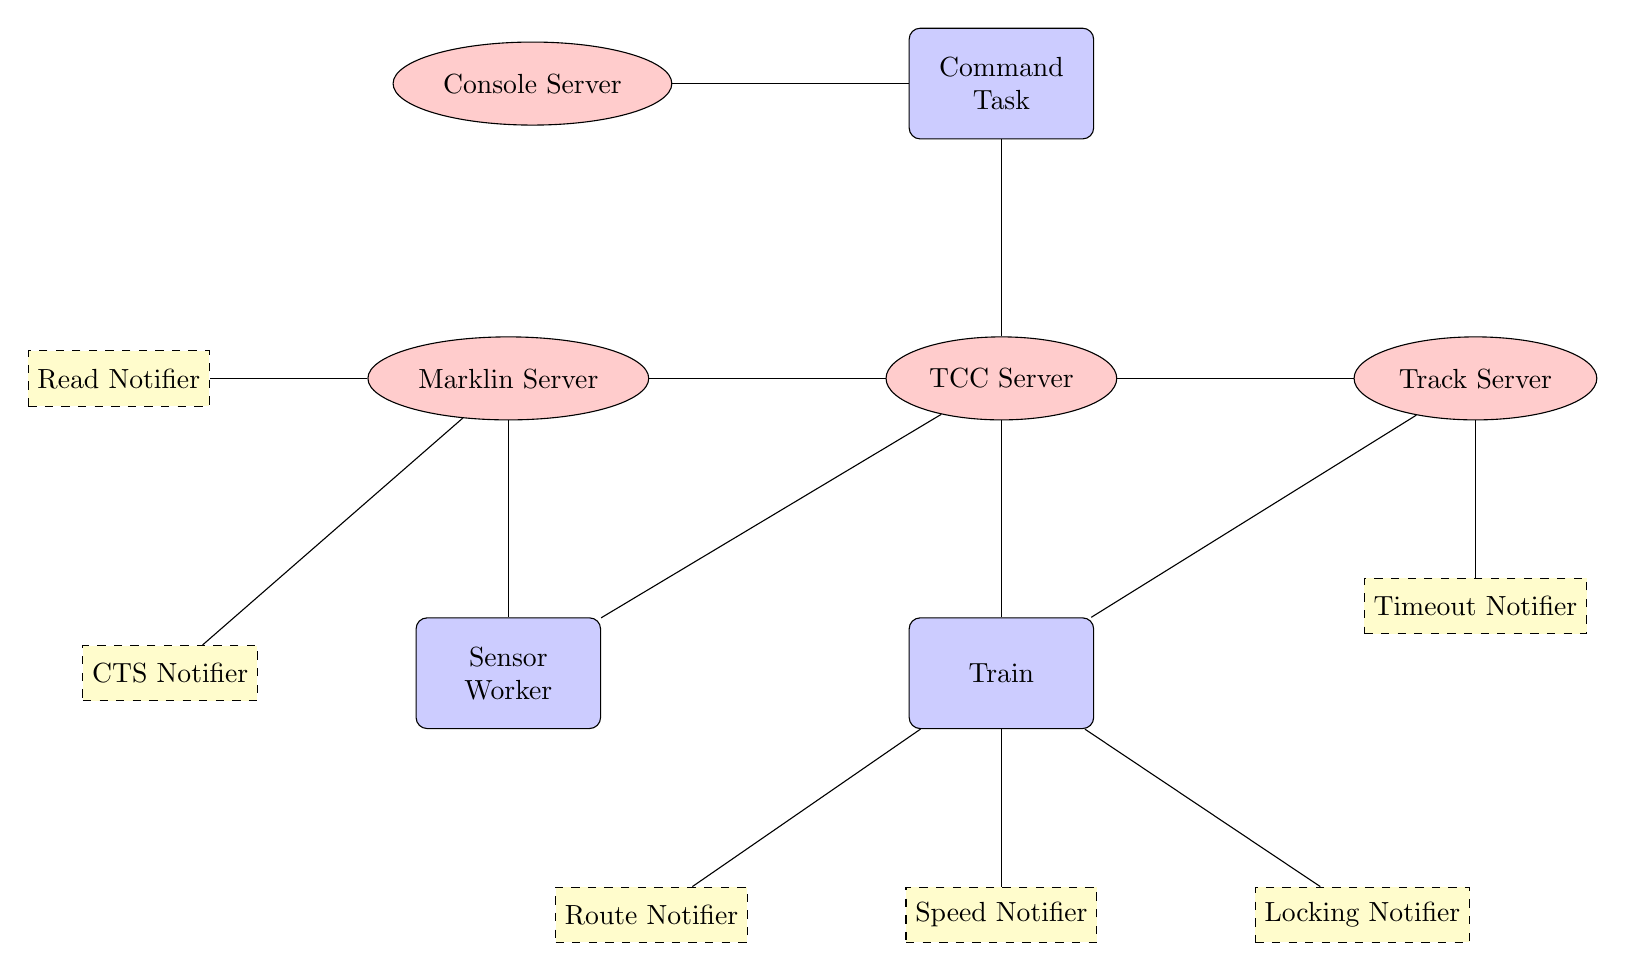
\begin{tikzpicture}[node distance=2.5cm and 3.5cm, auto]

        % Define styles
        \tikzstyle{block} = [rectangle, draw, fill=blue!20, text width=6em, text centered, rounded corners, minimum height=4em]
        \tikzstyle{cloud} = [draw, ellipse,fill=red!20, node distance=3cm, minimum height=3em]
        \tikzstyle{line} = [draw]
        \tikzstyle{notif} = [draw, rectangle, dashed, fill=yellow!20, node distance=2cm, minimum height=2em, text centered]
    
        % Place nodes
        \node [cloud] (marklin) {Marklin Server};
        \node [block, below=of marklin] (sensorworker) {Sensor Worker};
        \node [cloud, right=of marklin] (tcc) {TCC Server};
        \node [block, above=of tcc] (program) {Command Task};
        \node [cloud, left=of program] (console) {Console Server};
        \node [block, below=of tcc] (train) {Train};
        \node [cloud, right=of tcc] (track) {Track Server};
    
        % Notifiers
        \node [notif, left=of marklin] (Read) {Read Notifier};
        \node [notif, left=of sensorworker] (ctsnotif) {CTS Notifier};
        \node [notif, below=of train] (speednotif) {Speed Notifier};
        \node [notif, left=of speednotif] (routenotif) {Route Notifier};
        \node [notif, right=of speednotif] (locknotif) {Locking Notifier};
        \node [notif, below=of track] (timeoutnotif) {Timeout Notifier};
    
        % Draw edges
        \path [line] (console) -- (program);
        \path [line] (marklin) -- (sensorworker);
        \path [line] (marklin) -- (tcc);
        \path [line] (sensorworker) -- (tcc);
        \path [line] (tcc) -- (train);
        \path [line] (program) -- (tcc);
        \path [line] (track) -- (tcc);
        \path [line] (track) -- (train);
        
        % Notifier connections
        \path [line] (Read) -- (marklin);
        \path [line] (ctsnotif) -- (marklin);
        \path [line] (speednotif) -- (train);
        \path [line] (routenotif) -- (train);
        \path [line] (locknotif) -- (train);
        \path [line] (timeoutnotif) -- (track);
    
    \end{tikzpicture}
    }
    \caption{Train Control Tasks}
    \end{figure}
    
    \subsection{Position Modelling}
    \label{sec:positioning}
    
    In TC1, our implementation of position modelling supported only sensor predictions at constant speed. In order to enable sensor robustness (Section \ref{sec:sensor-robustness}), we required model the expected trigger time for the next sensor in all cases (i.e. including acceleration). We make these sensor predictions in the \verb`trn_position` class for each train, which is maintained by the Track Control Coordinator. This class implements a finite state machine for each train based on if it is currently waiting for a sensor (i.e. the TCC calls the \verb`trn_position_set_sensor` method), or if it has just hit the sensor it was previously waiting for (i.e. the TCC calls the \verb`trn_position_reached_sensor` method). Finally, the finite state machine has a third transition which may be started by the \verb`trn_position_update_speed`, which initialises the new non-constant speed prediction mode.
    
    First, for the constant speed case. This has not effectively changed from TC1, but has been adapted to better fit the more complex acceleration/deceleration scenario. When a train waits for a sensor, it passes the distance to its next sensor to the TCC, and by extension the positioning class. Using this value, it calculates the time expected to travel the given distance at the current speed, and saves it in the state. For any prediction, we make sure to buffer the old prediction value for when we hit the last predicted sensor. Finally, when we hit the sensor, are able to display this buffered prediction value along with the difference, as well as save the time that the sensor was activated, for handling acceleration.
    
    Acceleration begins and ends with the \verb`trn_position_update_speed` method. This is called by the TCC whenever trains send a speed request. The convention used is that if the train has reached its final speed (post acceleration/deceleration), it calls the speed set method with this final speed. This informs the FSM to allow it to transition back to the constant speed case, and reset any state which was held during the acceleration process. This is pre-calculated by the routing algorithm based on our models (see TC1 documentation for specific modelling methods). However, if the given speed is for a new speed, we transition to the acceleration state.
    
    In the acceleration state, we have two cases -- either we are stopped, or we are already moving. If we are stopped, since our position to the next sensor is unknown, there is no calculation we can do, so this next sensor has no expected time. Because of this, we only store metadata about the speed, and calculate the total distance of our acceleration using our modelling, in order to correctly end the acceleration state. We also use this time that the acceleration started as our \verb`last_timestamp` in lieu of any previous sensor activation. The second case occurs when we are already moving on the track. In this case, we use this last timestamp $t_\text{prev}$ and the timestamp of the speed change $t_a$ to calculate the relative time delta spend between the sensors travelling at constant speed as $\Delta t_\text{const} = t_a - t_\text{prev}$, and uses the previous estimate for when we would reach the next sensor to estimate the time remaining if we were  continuing at constant speed, denoted $\Delta t_\text{remaining-const} = \Delta t_\text{estimate} - \Delta t_\text{const}$. Using this, we calculate the distance remaining as
    \[
        \Delta d_\text{to-sensor} = \frac{v_0}{\Delta t_\text{remaining-const}}.
    \]
    Thus, using this remaining distance, we are able to model the time it will take us to accelerate over this distance, with our final speed unknown (since we could reach our desired velocity $v$ at any point in relation to the next sensor. This is calculated via the quadratic formula as
    \[
        \Delta t_\text{remaining} = \frac{-v_0 \pm \sqrt{v_0^2 + 2a\Delta d_\text{to-sensor}}}{a}, \numeq\label{eq:estimate_initial_accel}
    \]
    obviously taking only positive results. Using this new remaining time, we are able to adjust any existing sensor estimates by using
    \[
        t_\text{prev} - \Delta t_\text{remaining-const} + \Delta t_\text{remaining}
    \]
    as our new absolute timestamp estimate. Note that this estimate may be queued depending on the state of the positioning algorithm. In order to have all the information to make this new prediction, we queue this update so that the above recalculations occur after the train administrator has stated it's intentions for the next sensor (by waiting). This is needed since speed and routing are separate domains of the train administrator.
    
    Moreover, the calculation above for acceleration makes no assumptions that we were travelling at constant speed for the entire duration after hitting the previous sensor. This is particularly important for the case where we have multiple accelerations in a row. It only makes the assumption that we are at the constant speed, which is generally a safe assumption to make, and attempted to be guaranteed by our trains.
    
    Normally, when a train waits for the next sensor in the path, the positioning algorithm makes its next prediction. However, in the case that we have just started up, we cannot do so, since we still don't know the distance between train and the starting node when the train was started (at least in the constant case). However, we make this next prediction by using the distance $\Delta d_\text{travelled}$ we have already travelled over the acceleration phase prior to the last hit sensor and the distance to the next sensor given by the routing algorithm $\Delta d_\text{to-next-sensor}$ in the same formula as \eqref{eq:estimate_initial_accel} to find the total time we will have travelled by the next sensor:
    \[
        \Delta t_\text{total-at-next-sensor} = \frac{-v_0 \pm \sqrt{v_0^2 + 2a(\Delta d_\text{travelled} + \Delta d_\text{to-next-sensor})}}{a}.
    \]
    Using this calculated value, and the accumulated $\Delta t_\text{total}$, we can calculate the next expected sensor activation as $\Delta t_\text{total at next sensor} - \Delta t_\text{total}$.
    
    In the constant case, for the deferred prediction, we make the same calculation, but first need to calculate the distance between the train and the first sensor. Since we defer the prediction, we can calculate the relative time between acceleration and hitting said sensor, since both absolute timestamps are required as part of both methods, denoted $\Delta t_\text{pre-sensor}$. Using this, we are able to estimate this initial distance as
    \[
        \Delta d_\text{pre-sensor} = v_0 \Delta t_\text{pre-sensor} + \frac{1}{2} a \Delta t_\text{pre-sensor}^2.
    \]
    
    Finally, the terminating case (i.e. reaching constant velocity). We are able to recognise we are in this case when our total travelled distance so far ($\Delta d_\text{travelled}$), plus the distance to the next sensor ($\Delta d_\text{to-next-sensor}$) exceeds the pre-calculated total acceleration distance ($\Delta d_\text{total}$), i.e. $\Delta d_\text{travelled} + \Delta d_\text{to-next-sensor} > \Delta d_\text{total}$. In this case, we must calculate the expected time in first the non-constant case, and then the constant case. First, we calculate $\Delta d_\text{acceleration} = \Delta d_\text{total} - d_\text{travelled}$, the distance travelled in between these final sensors while accelerating. Then, we can trivially calculate $\Delta d_\text{const} = \Delta d_\text{to-next-sensor} - d_\text{acceleration}$. Then, all that remains is to calculate the time spent over each distance. For the acceleration distance, we can again use the quadratic formula to calculate
    \[
        \Delta t_\text{acceleration} = \frac{v \pm \sqrt{v^2 - 2a\Delta d_\text{acceleration}}}{a},
    \]
    and the calculation of $\Delta t_\text{const}$ is the same as always.
    
    In all cases, the work done when the train hits the expected sensor is very little. It consists only of displaying the difference to the UI and resetting/updating any necessary markers used during the actual calculations above.
    
    \subsubsection{Limitations}
    \label{sec:limits}
    
    We were unable to integrate the debug method with the sensor queue for resetting expected times. If we had been able to do so, in conjunction with the Sensor Robustness resetting, our modelling and sensor robustness would have been resilient to the decision point emergency stopping (Section \ref{sec:train}), allowing us to enter an unknown state before recovering, similar to the state after the train starts from a stationary position. Without these reset methods, our sensor-robustness and positioning failed due to the emergency stop, since it was not made aware that the train had stopped, and thus the expected time of the sensors could be changed to be ignored, as done initially on start-up.
    
    \subsubsection{Square Roots}
    
    The keen-eyed reader may have noticed that many of the modelling above required solving the problem of finding the square root. Without the C stdlib \verb`math.h` header, we implemented our own algorithm for efficiently calculating the integer square root of a number. We used Newton's Method for approximating solutions to the equation $x^2 - a$ to calculate the integer approximation for $\sqrt a$, using
    \[
        x_{n+1} = \frac{1}{2}\left(x_n + \frac{a}{x_n}\right)
    \]
    as our next estimate, and finishing when we were unable to keep refining, since we did not have floating point numbers.
    
    \subsection{Train Administrator}
    \label{sec:train}
    
    The Train Administrators for TC2 share the same general structure as those of TC1 in terms of notifiers and execution methods, but differ in two ways. Firstly, each administrator has a \verb`locking_notifier`, which acquires proceeding segment locks on behalf of the train, since this requires blocking first for the first node in the segments, and then blocking at the locking server for at most the specified decision point time attempting to acquire the segment. In the timeout case, this notifier is also responsible for emergency stopping the train, similar to the speed notifier in TC1 (and still in this part).
    
    Moreover, the Train Administrator is also responsible for freeing any segments that it leaves. When the route notifier is told by the Track Control Coordinator that we have hit a sensor, we free the previous segment (found in the track data). Moreover, whenever the train stops, in order to reduce the parts of the track reserved (since we always have at least two segments of track reserved), it also frees any segments which it is not occupying on stopping (including when we reach the destination). This is done atomically at the locking server level, in order to prevent any race conditions.
    
    The second change to the Train Administrators is related to the changes made to the routing algorithm (Section \ref{sec:routing}). Since the route planning is now incremental, we need to constantly plan a new route to the destination based on our current position in the track. The Train also has to take into account the current speed state of the track. If the train is stopped, it attempts to plan a route in either direction (if available -- if a train is at against an exit/entry node, it will only have one single direction), and based on the segments necessary to proceed which are returned by the routing algorithm for each direction, it performs a blocking wait on either group of segments (see \ref{sec:locking}). When one group of segments become completely free, the locking server unblocks it, and gives it ownership of the segments. 
    
    The train then proceeds to the moving state. In this state, we first plan the route of our next segment, if it exists. We are able to get the starting node of this next segment from our current in-progress route. This next segment will not exist if we will reach the specified end node in our current iteration. If it does exist, it then attempts to acquire these next segments with a timeout via the \verb`locking_notifier`. If it is able to acquire the next segments, it immediately throws any switches (which are at the front of the path now) to ensure that when we do enter the segments, we will be able to proceed. Otherwise, the train returns to the first stopped state and the process repeats. Any other actions such as the routing and speed actions from TC1 remain the same. The state machine then exits when we have executed the final segment and stopped at our destination, ready for any further routing commands.


    \section{Sensor Attribution}
    \label{sec:sensor-attribution}
    
    Sensor Attribution is accomplished via segment locking (Section \ref{sec:locking}). Because we require that each train's administrator task has acquired the respective lock before a train can be in a segment of the track, any sensor activations which occur while a train has the mutual exclusion of sensors in the segment must have been made by the train holding the lock. Moreover, as in TC1, since trains wait on individual locks, spurious non-waited sensors do not affect train progress, and are ignored.
    
    \subsection{Sensor Robustness}
    \label{sec:sensor-robustness}
    
    In order to implement any kind of sensor robustness into our program, we required to be able to model with accuracy the expected next activation time of a sensor (Section \ref{sec:positioning}). As described in the TC1, we use a sensor queue to keep track of tasks waiting for various sensor activations. This was augmented to include time-based priority for the expected time. As part of our positioning algorithm, when we wait for a sensor, it almost always returns the expected time that we activate said sensor based on the existing state of the track. If it is unable to, the sensor is waited upon without a time, and ignored for timeout calculations. In this case, the positioning algorithm may update the expected time that the sensor will be activated. Our sensor worker task, which polls the Märklin for sensor data, also periodically wakes up the sensor queue to check for any timeouts (i.e. have we missed the expected time of a sensor, with a grace period).

    Our sensor queue was also changed to maintain a simple state machine to handle the following possible scenarios for sensor activation:
    \begin{enumerate}
        \item On-time sensor activation;
        \item Unexpected sensor activation;
        \item Early sensor activation;
        \item Late or missing sensor activation.
    \end{enumerate}
    
    An on-time sensor activation is a sensor activation which occurs within an acceptable window of the calculated expected time ($\pm$200 ms), or a sensor that was waited upon without an expected time. We determined this window since we found that most of our predictions tended to lie within this interval on activation.
    
    An unexpected sensor activation occurs when a sensor is activated without any trains waiting on it. Due to the dynamic routing and on-the-fly switching our program uses to control trains, random sensor attributions are almost impossible to attribute to any particular train. An unexpected sensor activation may have been a false activation, or a malicious actor physically flicking switches on the track, in which case they can be ignored. Otherwise, this may be due to a train taking an unexpected route due to a malfunctioning or late switch. In this case, the train will miss its expected next sensor. Thus, this second case is handled in the late/missing sensor activation case, and we are able to just ignore any unexpected sensor activations.
    
    An early sensor activation occurs when a waited-upon sensor is triggered earlier than the expected window. This could be an incorrect activation, or an inaccurate prediction. In this case, we transition to an early error checking state. If the next sensor activation comes on time, we are able to assume the first prediction was just inaccurate, which can happen if the train gets stuck on the track, and thus return back the normal state. However, if this next sensor activation is also inaccurate (i.e. unexpected, early, late, or missing), we assume there is something wrong with the train and general state of train control, and we stop the train.

    A late sensor activation occurs when the sensor is triggered later than the expected window. This is treated in the same way as an early activation. However, in order to detect a late/missing sensor activation, we periodically check if there is a sensor we are waiting on that has not occurred, and is outside the window. As discussed above, we use the sensor worker to take over the role of a notifier to periodically wake the sensor queue up even without a sensor activation. As in the previous case, we also stop the train after two missing/faulty sensor activations.
    
    Unfortunately, our positioning algorithm was unable to properly recover after an emergency stop due to trains being unable to acquire their locks (Section \ref{sec:limits}). This caused an infinite cycle of faulty predictions causing trains to be stopped even after performing the expected action. This scenario only occured with multiple trains on the track, and without multiple sensor activations, our sensor robustness had no issues, but in order to demo the primary features of our program, we had to deactivate our sensor robustness algorithm for the demonstration.
    
    \section{Track Locking}
    \label{sec:locking}
    
    Rather than using any position-based avoidance algorithms, we prevent collisions by locking or reserving parts of the track.
    
    \subsection{Segments}
    
    In order to optimise the number of trains on parts of the track, we needed to choose segments appropriately to prevent multiple trains from colliding, while allowing necessary closeness in order for trains to route between various destinations. After exploring various methods, we decided to define a segment (or sector) as a section of the track without any escape routes for two trains in a head on collision, bounded on each exit and entry point by a sensor (if able, as in the case where a sector ends with an entry/exit node). This is illustrated in Figure \ref{fig:sectors}.
    \begin{figure}[h]
        \centering
        \includegraphics[width=0.9\textwidth]{nice-track-sectors}
        \caption{Track A Diagram with Sectors.}
        \label{fig:sectors}
    \end{figure}
    
    This choice has some drawbacks, particularly since the sizes of segments are quite uneven. For instance, some segments are as short as 20 cm, while others can cover up to four switches. Despite this uneven distribution, a significant advantage of this method is that we are able to precisely track when a train enters and exits a segment, eliminating the need for speculative positioning predictions.
    
    Using the above segments, we updated our track data nodes to include a \verb`segmentId` field, found in \verb`track-control/include/track-data.h`. This identifier simplifies the process of determining a node's corresponding segment, as this field points to the segment which lies in front of the track node. Merges and branches also are assigned the \verb`segmentId` of the sensors which it lies between. Since sensors are directional, this process is also natural. Consequentially, the sector which a train is exiting can be found by checking the segment of the reverse sensor.

    \subsection{Track Locking Server}
    
    In order to effectively manage segments, and guarantee that only one train in a segment at a time, we implemented a \emph{Track Server} to manage locking and unlocking of these segments. This server maintains an array detailing each segment and the specific train it is currently assigned to. The Track Server offers custom locking methods in order to facilitate segment locking for trains on the track, specifically for how we route trains (Section \ref{sec:routing}).
    
    First, callers can lock an entire array of segments. The server will only lock these segments if all of the requested are available, and otherwise blocks until all requested segments are available. This all-or-nothing approach helps us avoid deadlocks (Section \ref{sec:deadlock}). Since we use message passing and only respond when all locks are able to be acquired, this preserves atomicity.
    Callers can also lock either of two arrays of segments. This corresponds to the two directions of possible routes for a stopped train. The server attempts to lock any one of the arrays, enabling a train to concurrently wait for availability on two routes
    
    Both of the above functions can be called with timeout. When segments are locked with timeout, the server will unblock the caller after (at least) the timeout period has passed, returning a failure. This is how decision points (Section \ref{sec:decision-pts}) are implemented on the train side. The server uses a notifier on the timeout period, and returns failure to the caller.
    
    Callers are also able to free all locks which it holds, except potentially one. This is used to prevent a train from holding multiple segments on the track and blocking other trains when stopping. We allow a train to hold the segment it is currently in. This prevents the hold-and-wait scenario which can cause deadlocks (see Section \ref{sec:deadlock}). Segments are usually freed individually as the train exits segments.
    
    When a train attempts to lock segments, the server first checks if all are free, and if so, gives the train the desired locks, and marks it as owned by the train. Otherwise, it does not reply to the train, and whenever segments are freed, it checks if the freed segments are being waited upon, and if any train which was previously blocked is able to acquire all of the sectors, it is then given those sectors.

    \subsection{Deadlock Prevention}
    \label{sec:deadlock}
    
    In our design, we focused on deadlock avoidance instead of deadlock detection. To do so, trains acquiring locks followed conventions that made deadlocks impossible to occur.
    
    Trains in motion wait on lock availability with a timeout, and this timeout is pre-calculated to ensure that when a train is at this point, it has not crossed into any sectors which it does not own. If a train fails to acquire the next lock on its path, it executes an emergency stop, and frees all the locks it owns except the segment which the train is physically occupying. Timeout locking prevents an infinite block, and this atomic release prevents trains acquiring locks in the opposite order to enter a deadlock.
    
    Stopped trains also wait on two series of locks, corresponding to the forward and backwards routes, when able to move in that direction. This means that if there is an alternative route, trains will always take said alternative route, preventing any deadlock.
    
    This design philosophy works since in any place on the track, there will always be at least one train that can move backwards, physically backing out of any deadlock situations. Since stationary trains only maintain a lock on their physical position, one of these routes is always guaranteed to be unlocked.
    
\end{document}
